% why fixed-size?
% or are you saying that everyone does this, and then in the next paragraph, say that we do this too
% The reason is that both distance-based and density-based clustering algorithms work with fixed size datapoints.
The general idea for automatically finding the pervasive code patterns within a list of programs is to parse the programs and encode the important parts of the derived AST in fixed sized datapoints. Then, one uses a clustering algorithms to cluster these datapoints. Work in this vein makes the assumption that each cluster corresponds to one change pattern.

% put a footnote with the URL for Syn
% which APIs can't be used generally?
Our pipeline for finding pervasive patterns in Rust programs also follows this idea. We decided to implement our pipeline completely in Python. To make this work, we need a way to get an AST as a Python dictionary. Syn is a Rust crate which is designed to be employed in Rust procedural macros. However, it includes a parser which is suitable for our purposes; we simply had to write a preprocessor to transform Syn AST output into Python dictionaries.

A change pattern categorizes a class of changes. We thus need to define what a change is. For our purposes, a change is ....
To compute the contents of a change, we need two code revisions: the revision before the commit, and the revision after it. After parsing these two revisions, we will have two ASTs, encoded in two Python dictionaries. The change in the code can be computed by analyzing the difference of these two trees, which we call the ASTDiff. To derive the ASTDiff we use dictdiff Python library. 
% the wording in the two last sentences is inexact. Let's try to make clear exactly what the steps are, and use the right verbs.

An ASTDiff may include an arbitrary number of semantic changes. We are interested in finding the most important change within an ASTDiff and encoding that change in our datapoints. Sections ? and ? provide a detailed explanation of how we select the most important semantic information, which then helped us to effectively obtain meaningful clusters. % justification of that last assertion about meaningful clusters? e.g. we found that this helped us to effectively obtain meaningful clusters; but maybe we just don't know.

% why do we use pydriller?
% section N explains how we found the bug-related commits
We used Pydriller, which is a repository miner for Python. Our target repositories were the top 18 most starred open source Rust projects on GitHub. We mined all the bug related commits and ran them through our pipeline. Then, we applied the DBSCAN clustering algorithm on the obtained datapoints. In Section ? we discuss why we chose DBSCAN for clustering and how we tuned it to improve clusters quality. 

\subsection{Data modelling}

\subsubsection{Parsing Programs}

% TODO: tokens are not non terminals
% what do you mean about structs and enums?
% try to remove redundant content with respect to what is above
As mentioned above, we use Syn for parsing Rust. Syn handles all of Rust. Syn's nonterminals are primarily divided into two main groups; Structs and Enums. The dimensions of our datapoints have been designed in a way that it adheres to the nonterminals described in these two groups. We parse two versions of a Rust changed file in a commit; the file before the commit and after it. We will obtain two trees created by Syn. The change that transforms the first tree to the second one yields the fix which was applied in the commit. 

To find this difference, we use dictdiff, a Python library to find the diff of two Python dictionaries. Using the PLY tool (a Python implementation of lex and yacc), we wrote a simple transformer from the Rust AST into Python dictionaries. After obtaining the syntax trees in Python dictionary format, we can use dictdiff to determine the ASTDiff. 

dictdiff tool provides modifications' types: 
\begin{itemize}
\item `add': A new structure has been added to the tree; 
\item `remove': A structure has been dropped from the tree; 
\item `change': The content of a sub structure of the first tree has changed.
\end{itemize}
dictdiff also determines the context within which the modification has occured. This context happens to be the root elements (FIND A BETTER TERM FOR ROOT ELEMENTS) in our file, e.g. function blocks, struct blocks, impl blocks, etc. The modified content within a context is still in the form of tree. Our objective right now is to find primary elements in our diff that describe the semantics of occurred change.
% rework the above paragraph

\subsubsection{Path Linearization}

\begin{figure}[h]
\centering
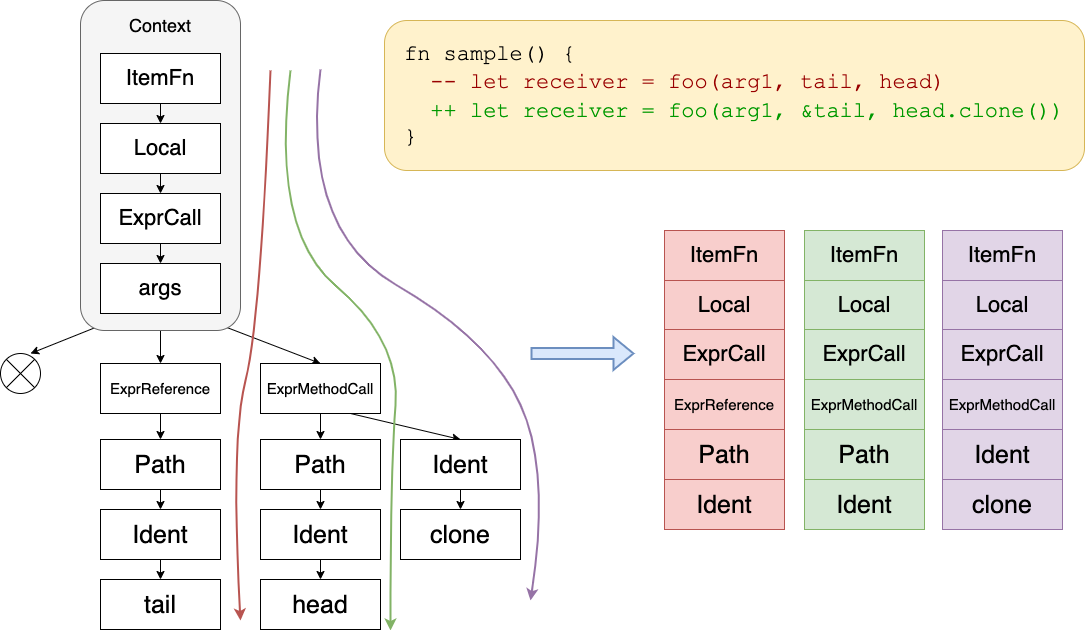
\includegraphics[width=0.8\textwidth]{linearization.png}
\label{f2}
\caption{Path Linearization}
\end{figure}

The output of dictdiff is a list of diffs, where each diff is constituted of three parts. The first part specifies whether the modification is of type 'add', 'remove', 'change'. The second part identifies the context of the modification, that is, the path from the root of the tree to the subtree in which the modification has occured. The third part is the content of the change and includes all the involved terminals and non terminals in the change. Our tool looks for changes within each root-level scope. That is, our assumption is that a change pattern occurs within one root-level scope. Our perspective does not cover the patterns that involve changes in multiple functions or multiple files. However, if the change happens in multiple lines within one scope, whether they are continuously one after another or separate from each other, our tool would be able to detect it.

Looking at the tree encoded in the content part of each diff, we realized that each path to a leaf represents one contributing element to the change. Through a Depth First Search we can collect all of these paths. We store only the non terminals that exist in the Syn token types list. Also certain keywords are not considered as non terminals in the syntax tree (e.g. clone, Box), but as they have a special meaning the language, we also store them in the path. The outcome of the DFS search is a set of linearized paths.

Fig \ref{f2} shows a simple change and its respective linearized paths. In the change, the second argument sends a borrow of the variable as opposed to sending the ownership entirely, and in the third argument, instead of sending the head into the function scope, we send a clone of it. A simplification of the derived diff of the two code revisions is shown in the figure. A DFS search on this tree would yield three different paths shown in three different colors. The path linearizes the hierarchy of non terminals involved in that specific path which represents one contributing factor to the change. We found it crucial to record the order of all non terminals involved in a path as it gives us freedom to control the degree of order-sensitiveness in our datapoint encoding.

The next question is how to transform these paths to a fixed size datapoint. First step, we need to define a fixed set of columns. The number of columns would depend on the amount of information we want to encode in the datapoints. The naivest approach would be to only report the observed non terminals within the diff. That yields a fully order-insensitive representation. In such encoding, for instance, there is no difference between two nested if statements and two if statements beside each other. Theoritically, to reach full order-sensitiveness, we would need encode all possible combinations of token types as our dimensions, which yields an astronomical number of dimensions. Apart from that, not all combinations adheres to Rust syntax. A reasonable work around would be to categorize the non terminals and set the dimensions as all possible combinations of these categories (Similar to JS paper, ref). This would reduce the number of dimensions and provide more reasonable and syntactically-correct combinations. However, after data collections we would still encounter a sparse dataset. 

In our methodology, similar to the first approach, we define the columns of our dataset, as the set of token types we collected from Syn. However, to achieve an acceptable level of order-sensitiveness, we carried out two auxiliary steps. Firstly, we record the number of occurrences of token types within the paths at each scope. The reason behind this decision is because different order of program elements yields a different number of occurrences of underlying token types. Secondly, we semi-automatically design a weighting scheme to give more value to certain non terminal we think are more important in Rust.

\subsubsection{Weighting Scheme}

Our main objective is that our datapoints manifest the change with high level of precision. For instance, the purple path in Fig \ref{f2} can be described as a change in local variable declaration, a change in a function call, calling a method of one of the function arguments, or calling clone() of one of the function arguments. Obviously, the last description is the most favorable one, as it offers the most accurate description. The whole idea behind our weighting scheme is to be able to identify the change accurately. 

A simple heuristic is that the closer we get to the leaves in the ASTDiff, the more important token types get. Another observation is that the elements closer to the root tend to be repeated in all the paths within one ASTDiff (Similar to ItemFn, Local, ExprCall in Fig \ref{f2}). Exploiting the latter observation, to obtain a basic knowledge about the number of repetitions of token types, we mined the last 20 bug related commits of the last 20 most starred rust projects on GitHub, and ran them through of pipeline. We recorded the number of occurrences of each token type in total. Then we gave the value of the inverse of the number of occurrences to each token. The intuition is that the higher the number of occurrences of a token type, the closer it is usually seen to the root. Hence, it probably does not provide us with the most accurate description of the change. In addition to that, as we wanted to make sure that our tool captures the patterns related to borrow checker, we manually raised the weights of the token types related to borrow checker. That is why we characterize our weighting scheme as semi-automatically designed. 

At last, each datapoint is created by the multiplying the number of occurrences of each token type to its weight and placing the result under its respective column. We call the set of final values the essence of the change, as we claim the values of token types manifest their importance in the change.

\subsection{Mining Repositories}

\begin{figure}[h]
\centering
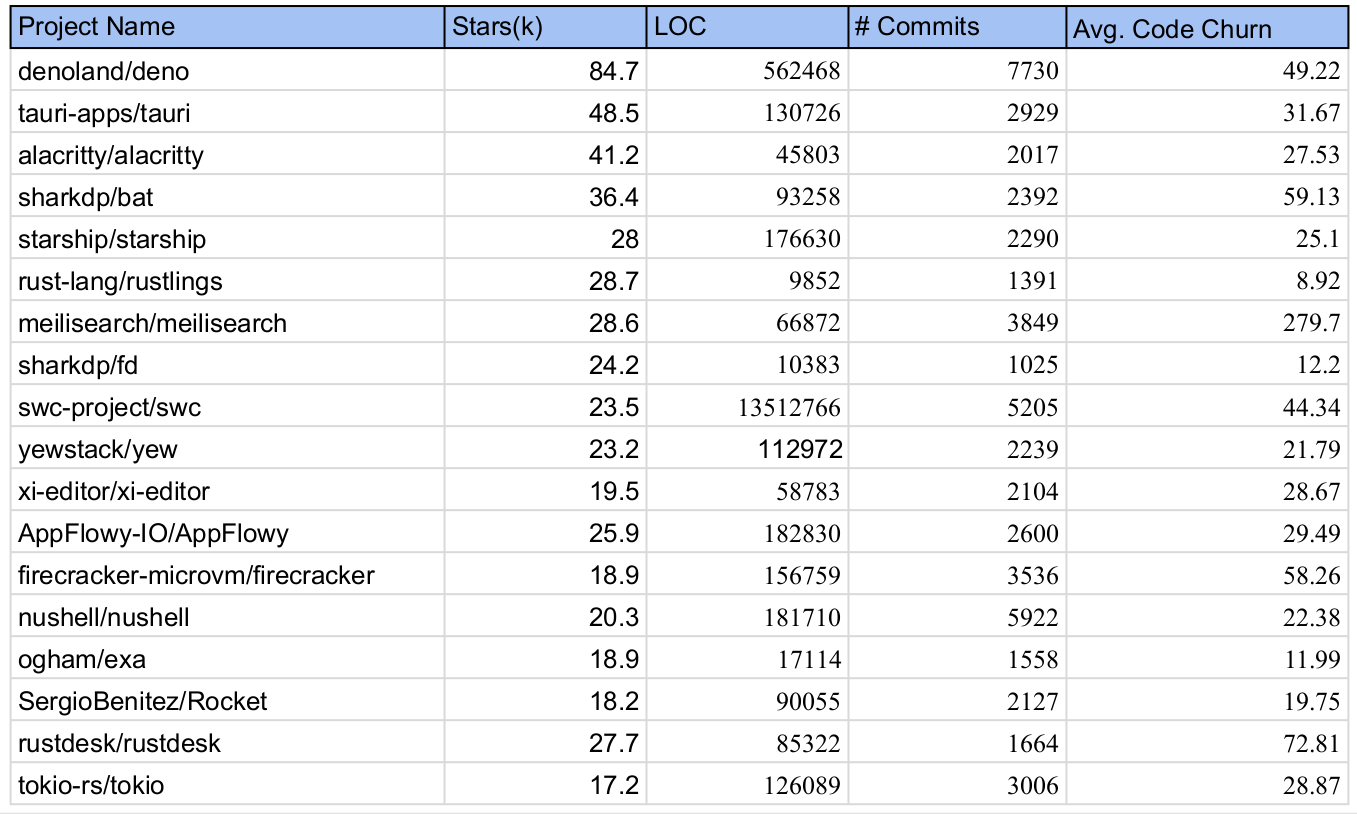
\includegraphics[width=1\textwidth]{repos.png}
\label{f3}
\caption{Target Repositories}
\end{figure}

Now that we have set up our code analysis pipeline, we can start mining the Rust repositories. We target the top 18 most starred Rust projects on GitHub, at the time of data collection. The details of these projects are outlined in Table \ref{f3}. We computed the average code churn of the files within the projects. denoland/deno and swc-project/swc are the projects with largest number of LOCs and average code churn. Unsurprisingly, we captured a lot of instances from these two projects in our final clusters.

\begin{algorithm}
\caption{An algorithm with caption}\label{alg:cap}
\hspace*{2mm} \textbf{Input:} $R$ (target repositories)  \\
\hspace*{2mm} \textbf{Output:} $D_g$ (General code changes) \\
\hspace*{2mm} \textbf{Output:} $D_b$ (BC-related code changes)
\begin{algorithmic}
\State $D_g \leftarrow \phi$
\State $D_b \leftarrow \phi$
\For{$r \in R$}
    \For{$c \in \textsc{ExtractCommits}(r)$}
        \If{$c.msg$ contains bug fixing related keywords}
            \For{$\{f_b, f_a\} \in \textsc{GetModifiedRustFiles}(c)$}
                \For{$e \in \textsc{ASTDiff}(\textsc{Parse}(f_b), \textsc{Parse}(f_a))$}
                    \State $DP \leftarrow \textsc{GetDataPoint}(e)$
                    \State $DP \leftarrow c.hash \cup f_a.name \cup e.scope \cup DP $
                    \If{$\textsc{IsBCRelated}(e)$}
                        \State $DP \leftarrow \textsc{GetBCKeyword}(e) \cup DP $
                        \State $D_b \leftarrow D_b \cup DP$
                    \Else
                        \State $D_g \leftarrow D_g \cup DP$
                    \EndIf
                \EndFor
            \EndFor
        \EndIf
    \EndFor
\EndFor
\end{algorithmic}
\end{algorithm}

%% Describing algorithm

\subsection{Clustering Data}

%% Why DBSCAN

%% Choosing Parameters

%% Figure

%% Manual Analysis for finding best parameter 

%% Final Clusters
